% EasyTeX feature test
% ---------------------------------------------------------------------------
% Open this file in EasyTeX and press Cmd+S. Each section below tests one
% feature and starts with a short "TRY:" note saying what to check.
% Sections 11 and 12 are switched off; remove the % signs to test them.
% ---------------------------------------------------------------------------
\documentclass[11pt,a4paper]{article}

\usepackage[T1]{fontenc}
\usepackage[utf8]{inputenc}
\usepackage{lmodern}
\usepackage{amsmath,amssymb}
\usepackage{graphicx}
\usepackage{booktabs}
\usepackage{xcolor}
\usepackage{tikz}
\usepackage{lipsum}
\usepackage[colorlinks=true,linkcolor=blue,citecolor=teal,urlcolor=magenta]{hyperref}

\title{EasyTeX Feature Test}
\author{Lorem Ipsum}
\date{\today}

\begin{document}
\maketitle
\tableofcontents
\newpage

% ===========================================================================
\section{Compile and PDF preview}\label{sec:compile}
% TRY: Cmd+S compiles. The PDF appears on the right and keeps its scroll
%      position when you compile again. Try the zoom buttons (- / fit / +).
Lorem ipsum dolor sit amet, consectetur adipiscing elit. Sed do eiusmod tempor
incididunt ut labore et dolore magna aliqua. Ut enim ad minim veniam, quis
nostrud exercitation ullamco laboris nisi ut aliquip ex ea commodo consequat.
Duis aute irure dolor in reprehenderit in voluptate velit esse cillum dolore eu
fugiat nulla pariatur.

% ===========================================================================
\section{Syntax highlighting}\label{sec:highlight}
% TRY: commands, braces, math and this comment should each have their own
%      colour. Switch macOS to dark mode: the editor theme should follow.
Excepteur sint occaecat \textbf{cupidatat non proident}, sunt in \emph{culpa qui
officia} deserunt mollit anim id est laborum. Inline math $a^2 + b^2 = c^2$,
a \textit{nested \textbf{bold} command}, and a 100\% escaped percent sign.

% ===========================================================================
\section{Auto-closing and completion}\label{sec:completion}
% TRY: on an empty line below, type \sec and pick "section" from the list.
%      Type { or [ or $ and the closing partner should appear. Select a word
%      and type { to wrap it in braces. Type \begin and pick an environment.
Curabitur pretium tincidunt lacus. Nulla gravida orci a odio. Nullam varius,
turpis et commodo pharetra, est eros bibendum elit, nec luctus magna felis
sollicitudin mauris.

% ===========================================================================
\section{Comment toggling}\label{sec:comments}
% TRY: put the cursor on the next text line and press Cmd+/ to comment it
%      out, then press Cmd+/ again to bring it back.
Integer in mauris eu nibh euismod gravida. Duis ac tellus et risus vulputate
vehicula. Donec lobortis risus a elit.

% ===========================================================================
\section{Mathematics}\label{sec:math}
% TRY: the equations compile and are numbered. Put the cursor on an
%      equation line and press Cmd+J to jump to the same spot in the PDF.
Etiam tempor. Ut ullamcorper, ligula eu tempor congue, eros est euismod turpis:
\begin{equation}\label{eq:gauss}
  \int_{-\infty}^{\infty} e^{-x^2}\,dx = \sqrt{\pi}
\end{equation}
\begin{align}
  f(x) &= \sum_{n=0}^{\infty} \frac{f^{(n)}(a)}{n!}\,(x-a)^n \label{eq:taylor}\\
  \nabla \times \mathbf{E} &= -\frac{\partial \mathbf{B}}{\partial t}
\end{align}
A matrix, just because:
\[
  A = \begin{pmatrix} 1 & 2 & 3\\ 4 & 5 & 6\\ 7 & 8 & 9 \end{pmatrix},
  \qquad \det(A) = 0,
  \qquad \mathbb{R}^n \subseteq \mathbb{C}^n .
\]

% ===========================================================================
\section{Lists and tables}\label{sec:lists}
% TRY: nothing special; checks common environments.
\begin{itemize}
  \item Lorem ipsum dolor sit amet.
  \item Consectetur adipiscing elit.
  \begin{enumerate}
    \item Sed do eiusmod tempor.
    \item Ut labore et dolore.
  \end{enumerate}
\end{itemize}

\begin{table}[h]
  \centering
  \caption{Lorem ipsum measurements}\label{tab:lorem}
  \begin{tabular}{lrr}
    \toprule
    Item & Dolor & Amet \\
    \midrule
    Lorem & 1.23 & 4.56 \\
    Ipsum & 7.89 & 0.12 \\
    Sit   & 3.45 & 6.78 \\
    \bottomrule
  \end{tabular}
\end{table}

% ===========================================================================
\section{Figures and images}\label{sec:figures}
% TRY: the image appears in the PDF. Click figures/easytex-icon.png in the
%      file tree: EasyTeX shows it as a preview instead of opening it as text.
\begin{figure}[h]
  \centering
  
\includegraphics[width=0.25\linewidth]{figures/easytex-icon.png}
  \caption{An image loaded from the \texttt{figures} folder.}\label{fig:icon}
\end{figure}

\begin{figure}[h]
  \centering
  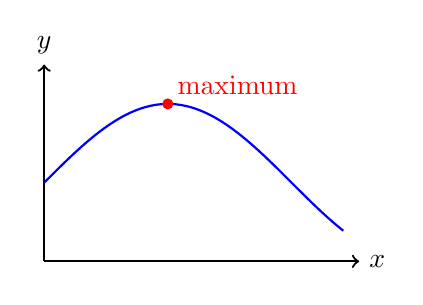
\begin{tikzpicture}
    \draw[thick,->] (0,0) -- (4,0) node[right] {$x$};
    \draw[thick,->] (0,0) -- (0,2.5) node[above] {$y$};
    \draw[blue,thick,domain=0:3.8,samples=60] plot (\x,{1+sin(\x r)});
    \fill[red] (1.57,2) circle (2pt) node[above right] {maximum};
  \end{tikzpicture}
  \caption{A TikZ drawing (needs the pgf package).}\label{fig:tikz}
\end{figure}

% ===========================================================================
\section{Cross-references, links and footnotes}\label{sec:refs}
% TRY: the numbers below are filled in after compiling (latexmk runs LaTeX
%      as often as needed). Links in the PDF are coloured and clickable.
See Section~\ref{sec:math}, Equation~\eqref{eq:gauss}, Table~\ref{tab:lorem},
Figure~\ref{fig:icon} and page~\pageref{sec:figures}. Visit
\url{https://www.ctan.org} or \href{https://www.latex-project.org}{the LaTeX
project}.\footnote{Lorem ipsum footnote. Phasellus viverra nulla ut metus.}

% ===========================================================================
\section{Bibliography}\label{sec:bib}
% TRY: the citations become numbers and the reference list appears at the
%      end (latexmk runs BibTeX for you). Open refs.bib to check its colours.
As shown by \cite{knuth84}, and later by \cite{lorem2020,vestibulum2023},
placeholder text is remarkably durable.

% ===========================================================================
\section{Files in sub-folders}\label{sec:input}
% TRY: the text below comes from chapters/feature-input.tex. Open that file
%      and press Cmd+S there: EasyTeX should still compile THIS file.
% This file is pulled into feature-test.tex with % This file is pulled into feature-test.tex with % This file is pulled into feature-test.tex with \input{chapters/feature-input}.
% Save it with Cmd+S: EasyTeX should find feature-test.tex through the
% "!TEX root" comment below and compile that instead of this file.
% !TEX root = ../feature-test.tex

\subsection{Text from a sub-folder}
Nam liber tempor cum soluta nobis eleifend option congue nihil imperdiet doming
id quod mazim placerat facer possim assum. This paragraph lives in
\texttt{chapters/feature-input.tex}. Double-click it in the PDF and the editor
should open this file at this line.
.
% Save it with Cmd+S: EasyTeX should find feature-test.tex through the
% "!TEX root" comment below and compile that instead of this file.
% !TEX root = ../feature-test.tex

\subsection{Text from a sub-folder}
Nam liber tempor cum soluta nobis eleifend option congue nihil imperdiet doming
id quod mazim placerat facer possim assum. This paragraph lives in
\texttt{chapters/feature-input.tex}. Double-click it in the PDF and the editor
should open this file at this line.
.
% Save it with Cmd+S: EasyTeX should find feature-test.tex through the
% "!TEX root" comment below and compile that instead of this file.
% !TEX root = ../feature-test.tex

\subsection{Text from a sub-folder}
Nam liber tempor cum soluta nobis eleifend option congue nihil imperdiet doming
id quod mazim placerat facer possim assum. This paragraph lives in
\texttt{chapters/feature-input.tex}. Double-click it in the PDF and the editor
should open this file at this line.


% ===========================================================================
\section{Long text for scrolling and SyncTeX}\label{sec:long}
% TRY: scroll the PDF to page 3 or 4 and double-click a word. The editor
%      should jump to the matching line here. Then put the cursor in a
%      paragraph below and press Cmd+J to jump the other way.
\lipsum[1-6]

% ===========================================================================
\section{Warnings}\label{sec:warnings}
% TRY: this reference points to a label that does not exist. After
%      compiling, the Problems panel (Shift+Cmd+L) lists a warning.
This reference is broken on purpose: Section~\ref{sec:does-not-exist}.

% ===========================================================================
\section{Errors (switched off)}\label{sec:errors}
% TRY: remove the % in front of the next line and press Cmd+S. The status
%      shows "1 error", the line is marked in the editor, and clicking the
%      error in the Problems panel jumps here. Put the % back afterwards.
% This line uses \thiscommanddoesnotexist on purpose.
Lorem ipsum dolor sit amet, the document still compiles without it.

% ===========================================================================
\section{Missing package (switched off)}\label{sec:missing}
% TRY: add the next line to the preamble (above \begin{document}). The
%      Problems panel reports the missing file. EasyTeX (Lite) also offers
%      to install real packages it can't find; PLUS already has them all.
% \usepackage{somepackagethatdoesnotexist}
Vivamus elementum semper nisi. Aenean vulputate eleifend tellus.

% ===========================================================================
\section{Special characters}\label{sec:unicode}
% TRY: typed directly as UTF-8; all should appear correctly in the PDF.
Umlaute: ä ö ü Ä Ö Ü ß. Accents: café, naïve, façade, señor, Øresund.
Quotes and dashes: ``lorem'' -- ipsum --- dolor. Euro: \texteuro\ is not in
every font, so this tests a TS1 symbol.

\bibliographystyle{plain}
\bibliography{refs}
\end{document}
